\documentclass[11pt]{article}
\usepackage[slovene]{babel}
\usepackage{hyperref}
\usepackage{siunitx}
\usepackage{xspace}
\usepackage{enumitem}
\usepackage{graphicx}
\usepackage{float}
\usepackage{url}

% !TeX spellcheck = sl_SL

\newcommand{\nina}{N.I.N.A.\@\xspace}

\title{Pripomočka za določanje obzorja in upoštevanje zgornje meje vidnega polja za mestno astrofotografijo}
\author{Jan Kalin $<$\href{mailto:jan.kalin@gmail.com}{jan.kalin@gmail.com}$>$}

\begin{document}

\maketitle

\section{Uvod}

Letos spomladi sem se navdušil nad astrofotografijo. Pri gledanju videov na YouTube in branju člankov izgledajo reči precej preproste. Vendar, kot je vsem verjetno jasno, traja nekaj časa da človek dobi rutino. Zato sem do sedaj 99\% fotografiranja opravil z domačega balkona. Ta pristop sicer pomeni precej večje udobje pri nabiranju znanja, ima pa dve pomanjkljivosti.

V mestu je prisotna precejšnja svetlobna onesnaženost. To se do določene mere lahko umili z uporabo ozkopasovnih filtrov, vendar se učinkom v ši\-ro\-ko\-pa\-sov\-nem območju skoraj ne da izogniti. Tolažim se z dejstvom da, ko bom enkrat znal dobiti dokaj dobre slike z balkona, bodo slike dobljene z dobrih lokacij se precej boljše.

Drugi problem je omejeno vidno polje. Konkretno, z mojega balkona je vidno nebo med azimutoma \SI{38}{\degree} in \SI{190}{\degree}, spodnja meja so hiše in drevesa, v nasprotju s fotografiranjem na odprtem pa tudi žleb na robu strehe.

Za kontrolo nosilca in kamere uporabljam aplikacijo \href{https://nighttime-imaging.eu/}{\nina}, ki ima možnost uporabe datoteke tipa \texttt{.hrz}, v katerih vrsticah so navedeni pari (azimut, višina) in ki jih \nina zna prikazati kot spodnjo mejo na diagramih. Vendar sta prisotni dve pomanjkljivosti.

Določanje parov (azimut, višina) je z uporabo ekvatorialnega nosilca za teleskop sitna, saj sta za spremembo enega izmed teh potrebni spremembi v rektascenziji in deklinaciji, včasih v ne-intuitivni kombinaciji. Bolj sitno je, da \nina nima vgrajenega mehanizma za omejitev pogleda navzgor.

Za omilitev sem razvil dva pripomočka, ki bosta predstavljena v tem prispevku.

\section{Pripomoček za določanje obzorja}

Python skripta \path{make_horizon.py} pomaga pri določanju obzorja tako, da omogoči kontrolo ekvatorialnega nosilca z uporabo horizontalnih koordinat.

Skripta trenutno deluje v Windows okolju (tako, kot \nina), dalo pa bi se jo verjetno preprosto adaptirati za Linux. Na PCju mora seveda biti inštaliran moderen Python, poleg tega pa se Python paket \texttt{win32com}, ki omogoča kontrolo nosilca. In, ne nazadnje, na nosilcu mora biti montirana kamera, priklopljena na PC in tam zagnana aplikacija, ki na zaslonu prikazuje trenutno sliko s kamere. Lahko pa se uporablja iskalo z rdečo piko ali kak drug način določanja orientacije nosilca.

Skripta deluje v dveh načinih. V prvem načinu se skripto pokliče s komandne vrstice z dvema številskima argumentoma, azimutom in višino. Skripta se priklopi na nosilec, izklopi vodenje, pretvori koordinati v ekvatorialni sistem in usmeri nosilec v tisto smer. To je morda bolj primerno za testiranje in za začetno usmeritev nosilca.

Drugi način je interaktiven, ta je bolj primeren za dejansko določanje obzorja. V tem (privzetem) načinu se odpre okno, ki pričakuje ukaze, zaključene s pritiskom na \texttt{<Enter>}. Ukazi so:

\begin{description}[itemsep=0pt, labelindent=1em]
	\item[$<$alt$>$ $<$az$>$:] Usmeri proti tem koordinatam, npr., \texttt{180 45}
	\item[u/d:] Povečaj ali zmanjšaj višino za en korak
	\item[l/r:] Povečaj ali zmanjšaj azimut za en korak
	\item[U/D:] Povečaj ali zmanjšaj višino za pet korakov
    \item[L/R:] Povečaj ali zmanjšaj azimut za pet korakov
    \item[step $<$deg$>$:] Nastavi korak na \texttt{deg} ločnih stopinj (privzeto 2)
    \item[$<$filename$>$:] Dodaj zadnji azimut/višino datoteki \texttt{filename.hrz}
    \item[q/quit:] Izhod iz programa
\end{description}

Določanje horizonta postane s tem pripomočkom precej preprosto. Sam sem po končanem postopku v datoteko dodal še začetni in končni par (37, 90) in (191, 90), eno ločno stopinjo pred in po dejanskima mejama vidnega območja. Ko vklopiš prikazovanje obzorja v postavki {\em Options $\rightarrow$ Astrometry $\rightarrow$ Custom horizon}, se tedaj na diagramu v \nina pojavita navpični črti, ki jasno določita območje vidljivosti objekta, npr., M33.

Podobno se omejitev zaradi strehe lahko oceni, ko s pripomočkom določiš pare (azimut, višina) za žleb. Tukaj je koristno biti malo konzervativen in usmeriti teleskop nekaj stopinj nižje od žleba, saj odboj svetlobe lahko pokvari sliko še preden žleb dejansko pride v kader.

\begin{figure}[H]
	\centering
	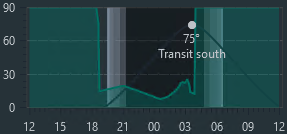
\includegraphics[width=0.45\textwidth]{floor.png} \hfill
	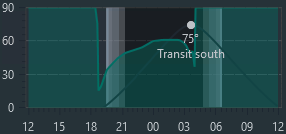
\includegraphics[width=0.45\textwidth]{ceil.png}
\end{figure}

Ta pripomoček je na voljo v \url{https://github.com/JanKalin/AstroRepo/tree/main/Python/horizon}

\section{Upoštevanje zgornje meje v \nina}	

Upoštevanje spodnje meje (obzorja) je vgrajeno v \nina v pogoju {\em Advanced Sequencer $\rightarrow$ Loop While Altitude Above Horizon}. Upoštevanje zgornje meja (streha) pa ni vgrajena, saj se pri uporabe \nina predpostavlja prost pogled v nebo. Zato sem razvil vtičnik, ki to omogoči omejitev pogleda navzgor.

Vtičnik se instalira v \nina preprosto tako, da se v direktoriju \path{C:\Users\<USERNAME>\AppData\Local\NINA\Plugins\3.0.0} kreira direktorij \path{Ceiling} in vanj prekopira datoteko \path{Ceiling.dll}. Po ponovnem zagonu \nina se bo med vtičniki pojavil {\em Ceiling}.

Uporaba je prav tako preprosta. V zaporedje ukazov v oknu {\em Sequencer $\rightarrow$ Advanced Sequencer} se na primerno mesto med {\em Loop Conditions} doda pogoj {\em Altitude Above Ceiling Limit}. Pogoj za pravilno uporabo vtičnika je izbira \path{.hrz}, datoteke v kateri je shranjena zgornja meja, npr., določena z \path{make_horizon.py}. Primer pravilno nastavljenega vtičnika je na naslednji sliki.

\begin{figure}[H]
	\centering
	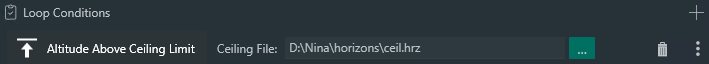
\includegraphics[width=\textwidth]{example.png} 
\end{figure}

Ko višina preseže mejo določeno v datoteki, se zajemanje slik ustavi, na zaslonu pa izpiše opozorilo:

\begin{figure}[H]
	\centering
	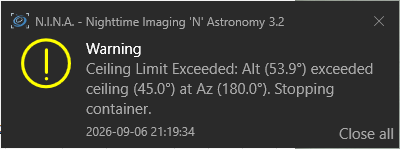
\includegraphics[width=0.5\textwidth]{warning.png} 
\end{figure}

Ta pripomoček je na voljo v \url{https://github.com/JanKalin/AstroRepo/tree/main/Nina/Plugins/Ceiling}. V osnovnem direktoriju je celotna izvorna koda, ki je prevedljiva z \texttt{.NET 8} SDKjem, v direktoriju \url{https://github.com/JanKalin/AstroRepo/tree/main/Nina/Plugins/Ceiling/bin/Release/net8.0-windows7.0} pa je že preveden vtičnik v datoteki \path{Ceiling.dll}.

\section{Testiranje}

Oba pripomočka sta bila narejena za osebno uporabo, licencirana sta z GPL3.0 licenco, ki omogoča prosto uporabo, širjenje, spremembe,\ldots da le ni v komercialne namene.

Ker sta oba pripomočka zelo nova, je seveda zelo možno, da so v obeh napake, ki se do sedaj niso pokazale. Če bo pri morebitni uporabi kdo naletel na napako, so povratne informacije zelo dobrodošle.

\end{document}